\pagenumbering{arabic}
\section{绪论}

\subsection{研究背景}

随着互联网的高速发展,人们生活在数字化的信息时代。相比以前较难获取信息,当下的人们可以十分便捷地接触到海量数据,以至于人们淹没在数据中难以快速的制定合适的决策。在校园中,学院的日常教务工作同样面临着这个难题,迫切地需要将已有的业务逻辑线上化。

其中,西安石油大学的毕业设计选题、中期检查、答辩等主要教学工作和学生工作,基本采用人工或半信息化的方式进行管理。针对这些陈旧的毕业管理工作,利用了新型网络技术,设计并实现毕业管理云平台系统,解决传统管理方式的效率低、工作量大、易出错等关键问题。

XSYU-GMS 系统是一个用于高校毕业生毕业流程线上管理的教务系统,由笔者独立开发,并于 2016 年起在西安石油大学计算机学院投入运行,承担了学院毕业设计选题工作。经过两年学院内测试后,该系统已基本完善,并且工作状态良好。本项目将在 GMS 系统的基础上进行二次开发,对接之前实现的毕业设计选题功能,实现毕业设计答辩系统。

\subsection{研究需求与意义}

本项目将使用新技术实现毕业设计答辩系统,解决在线下工作的不便以及存在的各种问题,同时新增大量特性以降低使用者的工作量。无论对于学生、教师还是管理人员,这套新系统都将会提供比以前更稳定易用的工作方式。

该项目使用了目前较为流行的 React 框架和 Node.js 后端技术,这样能使学生熟悉掌握目前比较新的 Web 开发技术。通过答辩系统项目的实践开发,学生可以混合使用在本科所学的多门学科,在实践中合理利用理论知识,提高学生在程序开发上的的动手能力。

本线上管理系统采用目前最新的 Web 开发技术搭建而成,具有可扩展、高可用性的特点,可以在后期根据需求开发新的模块。注重用户体验,完全按照学院规定的教学流程开发,方便教师学生使用。在之后可为西安石油大学计算机学院的教学管理工作定制开发,成为学院内与教务系统平行的一款教学辅助系统。

\subsection{研究现状及其前景}

几乎所有的高校都需要面对毕业生毕业设计、答辩的相关工作,基本没有学校再采用人工的方式进行管理。然而目前市面上并没有一款专门为此目的而开发的商业系统可供直接使用,大多数院校通过软件公司开发,或自己开发,这难免会造成功能不满足要求,或者开发质量低等问题。

部分学校所选用的教务系统或许有关于毕业设计的子模块,不过功能简单,还不足以满足学院教学工作的需要。目前对于毕业设计答辩流程的线上管理,将主要还是由各高校根据自己的相关需求,独立开发或外包开发。

类似的项目有阿尔巴尼亚高中设计的一个复杂的管理信息系统。该应用程序为其用户操作提供了一个合适的接口,以便简化和减少管理各个学校活动有关的信息和过程所需的时间。随着教育管理体制的深化和信息技术的进步,教育管理呈现出系统管理与教学管理脱节的趋势。该开发者认为,其根本原因在于教育管理体制整体建设的缺失。而山东师范大学信息科学与工程学院独立自主开发的“学生信息管理系统”软件,用于管理学生的学术数据。类似的,Norasiah et. al. 设计了一个学生档案管理系统 (SRMS) 信息系统 ,提供了一个直观的界面来管理学生数据。它能被很多大学或学院使用,以有效地记录学生的数据。它使用了序列图和状态图来详细分析数据的主要情况,然后给出系统的动态模型。并在教学管理系统面向对象建模的基础上,提出了一种设计过程。

尽管上述研究显示了一些让传统学生管理行业或行政管理所受益的项目,但仍不足以满足这种商业逻辑下的现代化要求。因此,我们需要开发一个更可靠的、更高性能的信息系统。


\subsection{传统 Web 开发技术简介}

在传统 Web 开发项目中,CGI(Common Gateway Interface)是能让 Web 服务器和 CGI 脚本正确处理客户的请求的协议。CGI 可以通过 C、PHP、Python、JSP 等多种编程语言实现。

如图 1-1 所示。其中 Web 服务器负责管理和维护来自用户的连接请求、基于 HTTP 协议的数据传输,以及网络交互等。CGI 程序则提供对具体的业务逻辑的实现。Web 服务器的功能主要是将客户端发来的 HTTP 请求转换成相应的 CGI 程序请求,然后执行目标程序,接着将 CGI 程序的输出作为结果,发送给客户端实现信息回复。

\begin{figure}
	\centering
	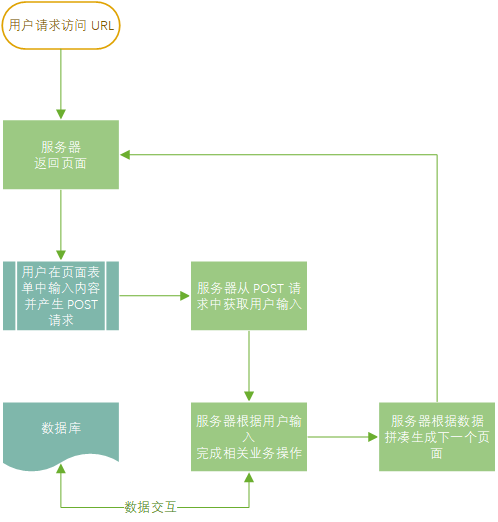
\includegraphics[width=0.7\linewidth]{figure/1-1}
	\caption{传统 Web 项目实现方式逻辑图}
\end{figure}

传统的 Web 开发,那都是由前端发送一个 HTTP 请求,一般包括 GET 请求和 POST 请求两种。后端处理该请求,并整理出 HTML 页面再返回。AJAX 也差不多,同样要经过发送请求、接收数据、写入页面的过程。应用逻辑都在后端,无数的请求往往成为开发的中心,但对于业务而言其实却是多余的。

除了数据传输时需要的封装请求和解析请求操作较为繁琐。我们还可以发现,页面的 UI 在后端产生,但又需要配合前端 CSS 进行维护,也可以在前端进行页面的二次修改,页面的显示逻辑分布在了前后端两侧,为项目维护造成了麻烦。

类似的情况发生在业务逻辑上,传统 Web 项目主要业务逻辑在后端完成。然而随着前端 JavaScript 的快速发展,很多简单逻辑被放在前端中执行。这虽然提升了项目开发效率,但同样带来了业务逻辑前后端分离的问题,在中大型项目中很容易会带来混乱,使项目不可维护。

RESTful(具象状态传输)架构是 Web 开发进一步发展后的成果,如图 1-2 所示。这是一种架构风格,它定义了一组基于HTTP的约束和属性。符合REST架构风格的Web服务提供了互联网上计算机系统之间的相互可操作性。符合REST的Web服务允许请求系统通过使用统一和预定义的一组无状态操作,来访问和操纵Web资源的文本表示(一般为 JSON 形式)。其他类型的Web服务有SOAP Web服务等。前端在获取静态的 HTML 页面之后,所有的业务逻辑和数据的获取操作均使用后端提供的 API 实现。在后端 API 保持不变的情况下,大部分业务逻辑在前端实现。这样使得项目开发更加规则,易于维护。但事实上,这种方式仍有少部分业务逻辑需要在后端实现。

\begin{figure}
	\centering
	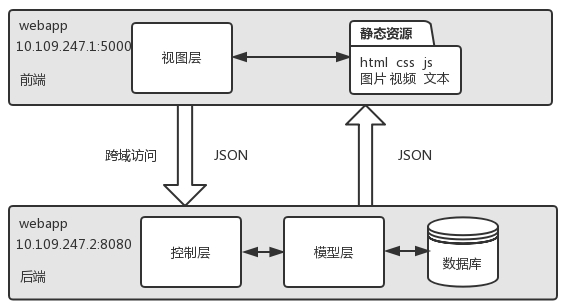
\includegraphics[width=0.7\linewidth]{figure/1-2}
	\caption{RESTful 架构开发方式}
\end{figure}

而本次答辩系统开发采用了更彻底地逻辑分离,在前后端分离的基础上抛弃了后端 API,几乎是直接暴露了后端数据库操作权限。消除了传统 Web 开发模式当中的请求封装、请求解析、拼装页面等一系列繁琐且多余的操作,集中在清晰的业务逻辑中,这有益于项目的快速开发和维护。

